\documentclass[12pt,letterpaper,oneside]{report}
\usepackage{fullpage,setspace,url,amsmath}
\usepackage{graphicx}
\usepackage{amssymb}
\usepackage{epstopdf}
\usepackage[parfill]{parskip}    
\usepackage[left=1in,right=1in,top=1in,bottom=1in]{geometry}

%%% Commands
\newcommand \groupname{Team Fuzzy Wuzzy}

\newcommand \code[1]{\texttt{#1}}
\newcommand \TODO[1]{\textbf{#1}}
\newcommand \qq[1]{``{#1}''}
\newcommand \etal{\textit{et al.}}

\renewcommand{\thesection}{\arabic{section}}


%%% Style
\bibliographystyle{ieeetr}
\usepackage[colorlinks=true, urlcolor=black, linkcolor=black, citecolor=black]{hyperref}


%%% Metadata
\title{Self-Organizing Map Character Recognizer}

%\subtitle{\groupname}
\author{ David Briscoe }


%%% Document
\begin{document}

% Front matter
\pagenumbering{roman}
\setcounter{page}{1}
%\setstretch{2}
\maketitle
\tableofcontents
\newpage

% Main matter
\setcounter{section}{0}
\pagenumbering{arabic}
\setcounter{page}{1}

\doublespacing


\section{Introduction}
% Explain some problem statements stuff here.
The purpose of this project was to develop a self-organizing map that would train on a selection of characters with different font faces and cluster them into groups corresponding to each letter. We consider the letters A to F.

\section{Objectives}
% State objectives of the project in excruciating detail, yay!
% Opportunities for citing references in absurd and wonderful ways?
%\cite{Ranjitkar}

\begin{enumerate}
\item Produce some input data
\item Provide a system to ensure the input data is the same form-factor so it can be accepted by the self-organizing map
\item Create an implementation of a self-organizing map that accepts a list of variables for inputs
\item Create a GUI that would allow the user to select an image of a letter to input into the self-organizing map and to display the output cluster.
\end{enumerate}

\clearpage
\section{Design and Implementation}
\subsection{Data and Data Normalization}
The input data are the letters A to F for three fonts. The fonts were selected at random, but novelty fonts were excluded. The fonts are Deja Vu Sans, Nimbus Roman, and Times New Roman. 

The fonts were taken from a word processor at 12 pt font and at 300\% zoom using a screen capture as shown in Figure \ref{fig:font-screengrab}. Each letter was separated and cropped to include no surrounding whitespace.

\begin{figure}[h]
  \centering
  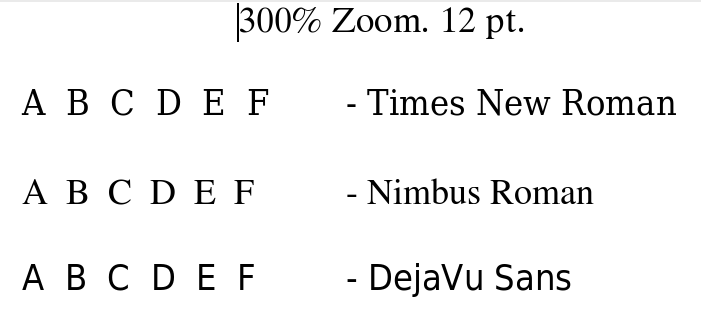
\includegraphics[width=5in]{diagrams/font-screengrab.png}
  \caption{The source for the fonts.}
  \label{fig:font-screengrab}
\end{figure}

The inputs are now roughly similar in size, but each pixel is represented by an RGB value. Also, the inputs must be the exact same size.

The inputs can be normalized by running them through \code{normalize.py} (\textit{See also Appendix \ref{apx:normalize}}). This program will convert them to greyscale and stretch them to all be the same size.


\subsection{Self-organizing map}
% Describe membership functions and how they were implemented in code
The self-organizing map is very straightforward. It contains a weight for each cluster. Each weight has the same number of elements as each input.

When training the self-organizing map, Euclidean distance is used to determine which weight is \qq{closest} to the input.


\subsection{Graphical User Interface}
% Describe the interface
The interface displays what the current input looks like and the current output of the self-organizing map. There are buttons to train the self-organizing map and to reset it back to its original (randomized) state. Figure \ref{fig:gui-plain} shows the interface.

\begin{figure}[h]
  \centering
  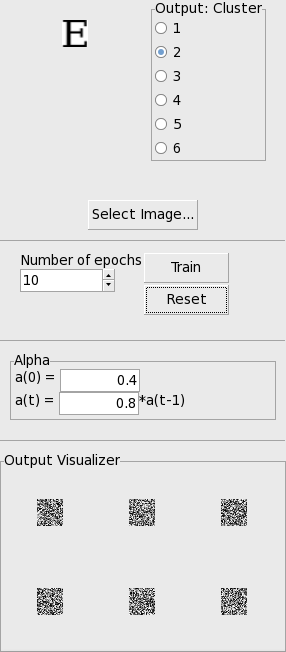
\includegraphics[width=2.5in]{diagrams/gui-plain.png} 
  \caption{The graphical user interface for inputting data into the self-organizing map.}
  \label{fig:gui-plain}
\end{figure}

The output displays the cluster that the self-organizing map has selected for the input image. The same input letter (with different or the same font face) should have the same cluster for its output.

The user can select a new image for input or train the self-organizing map.

Training will take all of the images in the \code{data} folder and pass them into the self-organizing map for the user's input number of epochs. The alpha function used for training is displayed in the bottom of the GUI. The user can modify the initial alpha or change the factor that alpha is scaled by on each training epoch. 


\clearpage
\section{Analysis}
% Analyze the results of our project...

\subsection{System before tuning}



\subsection{System after tuning}

\clearpage
\section{Appendix: Starting and Running the Application}\label{apx:running}
The application can be run as an executable using \texttt{python} at the command line.
Note that my application requires Python 2.5.

\subsection{Starting the Python Application}
\begin{enumerate}
  \item On a Windows system, open the \code{runapplication.bat} script. On a
      Unix-like system, open the \code{runapplication.sh} script.
  \item For more information see the README.txt file.
\end{enumerate}

\subsection{Guide to Running the Application}

\section{Appendix: normalize.py}\label{apx:running}

% Back matter
\bibliography{ref}

\end{document}
